%% using aastex version 6.3
%DIF LATEXDIFF DIFFERENCE FILE
%DIF DEL ../orig/FRB_struct_submit_Feb2023.tex   Mon Feb 13 17:42:07 2023
%DIF ADD FRB_struct_edited.tex                   Wed Oct 14 14:52:47 2026
%\documentclass[linenumbers]{aastex631}
\documentclass[twocolumn]{aastex631}



%\usepackage{siunitx}
\usepackage{tikz}
\usetikzlibrary{shapes,arrows}
\usepackage{graphicx}
\usepackage{amssymb}
\usepackage{subfigure}
\usepackage{epstopdf}
\usepackage{gensymb}
\usepackage{mathtools}
\usepackage{commath}
\usepackage{diagbox}
\usepackage{makecell}
\usepackage{CJKutf8} 
\usepackage{tabularx}% http://ctan.org/pkg/tabularx
\newcommand{\vdag}{(v)^\dagger}
\newcommand\aastex{AAS\TeX}
\newcommand\latex{La\TeX}
%\newcommand{\rev}[1]{\textcolor{blue}{#1}}
%\usepackage{comment}
%DIF 26a26
\newcommand{\Var}{\operatorname{Var}} %DIF > 
%DIF -------
\newcommand{\pccc}{\ensuremath{{\rm pc}\,{\rm cm}^{-3}}}

%%%%%%%%%%%%%%%%%%%%%%%%%%%%%%%%%%%%%%%%%%%%%%%%%%%%%%%%%%%%%%%%%%%%%%%%%%%%%%%%
\graphicspath{{./}{figures/}}
%DIF PREAMBLE EXTENSION ADDED BY LATEXDIFF
\RequirePackage[normalem]{ulem}\RequirePackage{color}\definecolor{RED}{rgb}{0.8,0,0}\definecolor{BLUE}{rgb}{0,0,0.85} %DIF PREAMBLE
\providecommand{\DIFadd}[1]{{\protect\color{BLUE}#1}} %DIF PREAMBLE
\providecommand{\DIFdel}[1]{{\protect\color{RED}#1}} %DIF PREAMBLE
\providecommand{\DIFaddbegin}{} \providecommand{\DIFaddend}{} %DIF PREAMBLE
\providecommand{\DIFdelbegin}{} \providecommand{\DIFdelend}{} %DIF PREAMBLE
\providecommand{\DIFmodbegin}{} \providecommand{\DIFmodend}{} %DIF PREAMBLE
\providecommand{\DIFaddFL}[1]{\DIFadd{#1}} \providecommand{\DIFdelFL}[1]{\DIFdel{#1}} %DIF PREAMBLE
\providecommand{\DIFaddbeginFL}{} \providecommand{\DIFaddendFL}{} %DIF PREAMBLE
\providecommand{\DIFdelbeginFL}{} \providecommand{\DIFdelendFL}{} %DIF PREAMBLE
\newcommand{\DIFscaledelfig}{0.5}
%DIF HIGHLIGHTGRAPHICS PREAMBLE %DIF PREAMBLE
\RequirePackage{settobox} %DIF PREAMBLE
\RequirePackage{letltxmacro} %DIF PREAMBLE
\newsavebox{\DIFdelgraphicsbox} %DIF PREAMBLE
\newlength{\DIFdelgraphicswidth} %DIF PREAMBLE
\newlength{\DIFdelgraphicsheight} %DIF PREAMBLE
% store original definition of \includegraphics %DIF PREAMBLE
\LetLtxMacro{\DIFOincludegraphics}{\includegraphics} %DIF PREAMBLE
\newcommand{\DIFaddincludegraphics}[2][]{{\color{blue}\fbox{\DIFOincludegraphics[#1]{#2}}}} %DIF PREAMBLE
\newcommand{\DIFdelincludegraphics}[2][]{% %DIF PREAMBLE
\sbox{\DIFdelgraphicsbox}{\DIFOincludegraphics[#1]{#2}}% %DIF PREAMBLE
\settoboxwidth{\DIFdelgraphicswidth}{\DIFdelgraphicsbox} %DIF PREAMBLE
\settoboxtotalheight{\DIFdelgraphicsheight}{\DIFdelgraphicsbox} %DIF PREAMBLE
\scalebox{\DIFscaledelfig}{% %DIF PREAMBLE
\parbox[b]{\DIFdelgraphicswidth}{\usebox{\DIFdelgraphicsbox}\\[-\baselineskip] \rule{\DIFdelgraphicswidth}{0em}}\llap{\resizebox{\DIFdelgraphicswidth}{\DIFdelgraphicsheight}{% %DIF PREAMBLE
\setlength{\unitlength}{\DIFdelgraphicswidth}% %DIF PREAMBLE
\begin{picture}(1,1)% %DIF PREAMBLE
\thicklines\linethickness{2pt} %DIF PREAMBLE
{\color[rgb]{1,0,0}\put(0,0){\framebox(1,1){}}}% %DIF PREAMBLE
{\color[rgb]{1,0,0}\put(0,0){\line( 1,1){1}}}% %DIF PREAMBLE
{\color[rgb]{1,0,0}\put(0,1){\line(1,-1){1}}}% %DIF PREAMBLE
\end{picture}% %DIF PREAMBLE
}\hspace*{3pt}}} %DIF PREAMBLE
} %DIF PREAMBLE
\LetLtxMacro{\DIFOaddbegin}{\DIFaddbegin} %DIF PREAMBLE
\LetLtxMacro{\DIFOaddend}{\DIFaddend} %DIF PREAMBLE
\LetLtxMacro{\DIFOdelbegin}{\DIFdelbegin} %DIF PREAMBLE
\LetLtxMacro{\DIFOdelend}{\DIFdelend} %DIF PREAMBLE
\DeclareRobustCommand{\DIFaddbegin}{\DIFOaddbegin \let\includegraphics\DIFaddincludegraphics} %DIF PREAMBLE
\DeclareRobustCommand{\DIFaddend}{\DIFOaddend \let\includegraphics\DIFOincludegraphics} %DIF PREAMBLE
\DeclareRobustCommand{\DIFdelbegin}{\DIFOdelbegin \let\includegraphics\DIFdelincludegraphics} %DIF PREAMBLE
\DeclareRobustCommand{\DIFdelend}{\DIFOaddend \let\includegraphics\DIFOincludegraphics} %DIF PREAMBLE
\LetLtxMacro{\DIFOaddbeginFL}{\DIFaddbeginFL} %DIF PREAMBLE
\LetLtxMacro{\DIFOaddendFL}{\DIFaddendFL} %DIF PREAMBLE
\LetLtxMacro{\DIFOdelbeginFL}{\DIFdelbeginFL} %DIF PREAMBLE
\LetLtxMacro{\DIFOdelendFL}{\DIFdelendFL} %DIF PREAMBLE
\DeclareRobustCommand{\DIFaddbeginFL}{\DIFOaddbeginFL \let\includegraphics\DIFaddincludegraphics} %DIF PREAMBLE
\DeclareRobustCommand{\DIFaddendFL}{\DIFOaddendFL \let\includegraphics\DIFOincludegraphics} %DIF PREAMBLE
\DeclareRobustCommand{\DIFdelbeginFL}{\DIFOdelbeginFL \let\includegraphics\DIFdelincludegraphics} %DIF PREAMBLE
\DeclareRobustCommand{\DIFdelendFL}{\DIFOaddendFL \let\includegraphics\DIFOincludegraphics} %DIF PREAMBLE
%DIF COLORLISTINGS PREAMBLE %DIF PREAMBLE
\RequirePackage{listings} %DIF PREAMBLE
\RequirePackage{color} %DIF PREAMBLE
\lstdefinelanguage{DIFcode}{ %DIF PREAMBLE
%DIF DIFCODE_UNDERLINE %DIF PREAMBLE
  moredelim=[il][\color{red}\sout]{\%DIF\ <\ }, %DIF PREAMBLE
  moredelim=[il][\color{blue}\uwave]{\%DIF\ >\ } %DIF PREAMBLE
} %DIF PREAMBLE
\lstdefinestyle{DIFverbatimstyle}{ %DIF PREAMBLE
	language=DIFcode, %DIF PREAMBLE
	basicstyle=\ttfamily, %DIF PREAMBLE
	columns=fullflexible, %DIF PREAMBLE
	keepspaces=true %DIF PREAMBLE
} %DIF PREAMBLE
\lstnewenvironment{DIFverbatim}{\lstset{style=DIFverbatimstyle}}{} %DIF PREAMBLE
\lstnewenvironment{DIFverbatim*}{\lstset{style=DIFverbatimstyle,showspaces=true}}{} %DIF PREAMBLE
%DIF END PREAMBLE EXTENSION ADDED BY LATEXDIFF

\begin{document}

\title{Calculation and Uncertainty of Fast Radio Burst Structure Based on Smoothed Data 
\footnote{Draft, \today}}


\author[0000-0002-9116-307X]{Adrian~T.~Sutinjo}
\affiliation{International Centre for Radio Astronomy Research, Curtin University, Bentley, WA 6102, Australia}

\author[0000-0002-6895-4156]{Danica~R.~Scott}
\affiliation{International Centre for Radio Astronomy Research, Curtin University, Bentley, WA 6102, Australia}

\author[0000-0002-6437-6176]{Clancy~W.~James}
\affiliation{International Centre for Radio Astronomy Research, Curtin University, Bentley, WA 6102, Australia}

\author[0000-0002-5067-8894]{Marcin Glowacki}
\affiliation{International Centre for Radio Astronomy Research, Curtin University, Bentley, WA 6102, Australia}

\author[0000-0003-2149-0363]{Keith W. Bannister}
\affiliation{ATNF, CSIRO, Space and Astronomy, PO Box 76, Epping, NSW 1710, Australia}

\author[0000-0002-2858-9481]{Hyerin Cho \begin{CJK}{UTF8}{}
 \CJKfamily{mj}(조혜린)\end{CJK}}
\affiliation{Center for Astrophysics $\vert$ Harvard \& Smithsonian, 60 Garden Street, Cambridge, MA 02138, USA}
\affiliation{Black Hole Initiative at Harvard University, 20 Garden Street, Cambridge, MA 02138, USA}

\author[0000-0002-8101-3027]{Cherie~K.~Day}
\affiliation{Centre for Astrophysics and Supercomputing, Swinburne University of Technology, Hawthorn, VIC, 3122, Australia}

\author[0000-0001-9434-3837]{Adam~T.~Deller}
\affiliation{Centre for Astrophysics and Supercomputing, Swinburne University of Technology, Hawthorn, VIC, 3122, Australia}

\author{Timothy~P.~Perrett}
\affiliation{International Centre for Radio Astronomy Research, Curtin University, Bentley, WA 6102, Australia}

\author[0000-0002-7285-6348]{Ryan~M.~Shannon}
\affiliation{Centre for Astrophysics and Supercomputing, Swinburne University of Technology, Hawthorn, VIC, 3122, Australia}


\begin{abstract}
Studies of the time-domain structure of fast radio bursts (FRBs) require an accurate estimate of the FRB dispersion measure in order to recover the intrinsic burst shape. Furthermore, the exact DM is itself of interest when studying the time-evolution of the medium through which multiple bursts from repeating FRBs propagate.
A commonly used approach to obtain the
dispersion measure is to take the value that maximizes the FRB structure in the time domain.
However, various authors use differing methods to obtain this structure parameter, and do not document the smoothing method used. Furthermore, there are no quantitative estimates of the error in this procedure in the FRB literature. In this letter, we present a smoothing filter based on the discrete cosine transform, and show that computing the structure parameter by summing the squares of the derivatives and taking the square root (that is, the 2-norm,  $\sqrt{\Sigma (d/dt)^2}$) immediately lends itself to calculation of uncertainty of the structure parameter. We illustrate this with FRB181112 and FRB210117 data, which were detected by the Australian Square Kilometre Array Pathfinder, and for which high-time-resolution data is available.

\end{abstract}


\keywords{
Radio transient sources (2008)---Astronomy data analysis (1858)
}


\section{Introduction} \label{sec:intro}

Fast radio bursts (FRBs) are extragalactic radio transients of millisecond duration~\citep{Lorimer2007}. Both the underlying mechanism of their emission, and the properties of the astrophysical plasmas through which they propagate, can be studied through detailed analysis of their time-frequency structure \citep[e.g.][]{Michilli2018_121102,Macquart2020}. The frequency dependent delay (dispersion measure, DM) of FRBs informs about the total integrated column density of free electrons --- and hence total matter density --- through which the FRB has propagated. Long-term studies of DM variation in repeating FRBs yield information on the medium in the vicinity of the progenitor \citep[e.g.][]{Zhao2021_DM_evolution}. Additionally, studies of FRB structure are sensitive to the assumed value of DM used to dedisperse the FRB \citep[e.g.][]{Hessels_2019}.
To this end, FRB analysis aims to identify the correct DM, i.e.\ that corresponding to the integrated electron column density through which the FRB has passed. While FRB searches use
the dispersion measure that maximizes signal-to-noise ratio (S/N),
it is often assumed that the correct DM is that which maximizes structure~\citep{Caleb_10.1093/mnras/staa1791, Hilmarsson_10.1093/mnras/stab2936, 2021MNRAS.505.3041P}.

A common measure of structure is the time-derivative of the pulse intensity $I(t)$~\citep{Gajjar_2018, Hessels_2019, Josephy_2019, Andersen2019, Pilia_2020}. However, since $I(t)$ is noisy, the derivative operation is not applied to a noisy estimate of the $I(t)$, but rather to a smoothed version thereof.
This smoothing operation has the potential to affect the structure-maximizing DM, since over-smoothing will smear out the intrinsic FRB structure, while under-smoothing will leave the derivative dominated by noise.  However, to date, there has been little attention paid on how to optimally select a smoothing time.

In the literature, there is also a slight variation in how the resulting $d/dt$ are combined. For example, \citet{Hessels_2019} used $\Sigma \left(d/dt\right)^2$, \citet{Gajjar_2018} suggested $\Sigma \left|d/dt\right|$, and \citet{Josephy_2019} experimented with $\Sigma \left(d/dt\right)^4$. One may argue that this is a matter of preference as long as the positive of the $d/dt$ is combined and an interesting structure is detected.
However, while any of these approaches should be able to identify the DM that maximises the structure in the signal, the uncertainty of the resultant fitted DM is also of considerable interest --- without an accurate estimate of this uncertainty, it is impossible to determine whether, for instance, the DM of a given source is changing between bursts.

In \secref{sec:method}, we shall demonstrate that the vector norm offers a meaningful measure of the uncertainty in the structure parameter inferred from noisy time-series data. In particular, the  $\sqrt{\Sigma (d/dt)^2}$ (Euclidean or 2-norm) offers a physical and intuitive interpretation, as illustrated in \secref{sec:result}. \secref{sec:apply} then illustrates how the structure parameter, and uncertainty thereon, to be calculated for two example FRBs. Under the assumption that the ``correct'' DM of an FRB\footnote{i.e.\ such that ${\rm DM}=\int n(e) (1+z)^{-1} d\ell$ for electron density $n(e)$ and unique signal propagation path $d \ell$.} is synonymous with structure maximization, this allows the correct DM to be identified, and assigned an uncertainty 
$\pm \Delta \text{DM}$ which quantifies the confidence in such a detection.

\section{Method} \label{sec:method}
\subsection{Matrix representation and uncertainty definition} \label{sec:unc_def}
Let $\mathbf{i}=[I(1),\cdots,I(N)]^T$ be a vector that contains discrete time samples of noisy total intensity $I(t)$. We may represent the smoothing operator as a matrix $\mathbf{S}$ and the first derivative as a matrix $\mathbf{D}_1$. Our immediate discussion here pertains to any $\mathbf{S}$ and $\mathbf{D}_1$ matrices, therefore the conclusions are generally applicable.  It suffices to say, as we shall demonstrate later, it is indeed possible to write the smoothing algorithm as a matrix; for example, see~\citet{Eilers_doi:10.1021/ac034173t, STICKEL2010467, Strang_wavelet}. The result of the smoothing process is the smoothed estimate
\begin{eqnarray}
\tilde{\mathbf{i}}=\mathbf{S}\mathbf{i}.
\label{eqn:smoothed}
\end{eqnarray}
The first derivative operator can be expressed as a matrix, for example, a simple forward difference on $N$ data points is a $(N-1) \times N$ matrix
\begin{eqnarray}
\mathbf{D}_1=
\left[ \begin{array}{c c c c} 
-1 & 1 &  &  \\ 
 & \ddots & \ddots & \\
   &   & -1 & ~1
\end{array} \right].
\label{eqn:D1}
\end{eqnarray}
Therefore, the first derivative of the smoothed data is 
\begin{eqnarray}
\mathbf{D}_1\tilde{\mathbf{i}}=\mathbf{D}_1\mathbf{S}\mathbf{i}.
\label{eqn:diff_smoothed}
\end{eqnarray}

The original noisy data can be expressed as the sum of the smoothed estimate and the difference between the noisy data and the smoothed version $\mathbf{\Delta_i}=\mathbf{i}-\tilde{\mathbf{i}}$. 
\begin{eqnarray}
\mathbf{i}=\tilde{\mathbf{i}}+\mathbf{\Delta_i}.
\label{eqn:i_Del}
\end{eqnarray}
\DIFaddbegin \DIFadd{Eq.~\eqref{eqn:i_Del} splits the data into estimates of the signal and the noise. The true parts are $\mathbf{i}=\mathbf{s}+\mathbf{n}$, with $\mathbf{s}$ the noiseless burst and $\mathbf{n}$ zero-mean noise with covariance ${\rm Cov}(\mathbf{n})=\langle\mathbf{n}\mathbf{n}^T\rangle$, where $\langle\cdot\rangle$ is the average over noise realisations. Since
}\begin{eqnarray}
\DIFadd{\mathbf{\Delta_i}=(\mathbf{s}-\mathbf{S}\mathbf{s})+(\mathbf{n}-\mathbf{S}\mathbf{n}),
\label{eqn:delta}
}\end{eqnarray}
\DIFadd{$\mathbf{\Delta_i}$ contains the burst structure that smoothing removes, and $\tilde{\mathbf{i}}=\mathbf{S}\mathbf{s}+\mathbf{S}\mathbf{n}$ contains the in-band noise $\mathbf{S}\mathbf{n}$ that smoothing cannot remove.
}\DIFaddend Therefore, Eq.~\eqref{eqn:diff_smoothed} may be written as
\begin{eqnarray}
\mathbf{D}_1\tilde{\mathbf{i}}&=&\mathbf{D}_1\mathbf{S}(\tilde{\mathbf{i}}+\mathbf{\Delta_i})\nonumber\\
&=&\mathbf{D}_1\mathbf{S}\tilde{\mathbf{i}}+\mathbf{D}_1\mathbf{S}\mathbf{\Delta_i}.
\label{eqn:D1_smoothed}
\end{eqnarray}
Eq.~\eqref{eqn:D1_smoothed} is illustrated in Fig.~\ref{fig:vec_sum}. We note that the first term in the right hand side of Eq.~\eqref{eqn:D1_smoothed}, $\mathbf{D}_1\mathbf{S}\tilde{\mathbf{i}}=\mathbf{D}_1\mathbf{S}\mathbf{S}\mathbf{i}$, is the derivative of the ``double-smoothed'' data. The second term, $\mathbf{D}_1\mathbf{S}\mathbf{\Delta_i}$, is the derivative of the smoothed ``de-trended'' noise. \DIFaddbegin \DIFadd{By Eq.~\eqref{eqn:delta}, however, the first term also contains in-band noise, and the second contains burst structure, $\mathbf{D}_1\mathbf{S}(\mathbf{s}-\mathbf{S}\mathbf{s})$. 
}\DIFaddend 

The length (2-norm, $\norm{.}_2$) of $\mathbf{D}_1\mathbf{S}\mathbf{\Delta_i}$ is the radius of the dashed circle in Fig.~\ref{fig:vec_sum}, which may be written as 
\begin{eqnarray}
\norm{\mathbf{D}_1\mathbf{S}\mathbf{\Delta_i}}_2=\sqrt{\sum_{n=1}^N \left[(\mathbf{D}_1\mathbf{S}\mathbf{i})_n-(\mathbf{D}_1\mathbf{S}\tilde{\mathbf{i}})_n\right]^2},
\label{eqn:norm_D1Si}
\end{eqnarray}
where $(.)_n$ indicates the $n$-th element of the vector in question. \DIFdelbegin \DIFdel{The right hand side of Eq. ~\eqref{eqn:norm_D1Si} suggests that it can be interpreted as proportional to a standard deviation estimate ($\tilde{\sigma}\sqrt{N-1}$)
of the first derivative of the smoothed data. Taking this as the uncertainty estimate of $\mathbf{D}_1\tilde{\mathbf{i}}$ means we take $\mathbf{D}_1\mathbf{S}\mathbf{\Delta_i}$ to represent a particular noise instance with standard deviation of $\norm{\mathbf{D}_1\mathbf{S}\mathbf{\Delta_i}}_2/\sqrt{N-1}$. In that case, the tip of the vector $\mathbf{D}_1\tilde{\mathbf{i}}$  in Fig.~\ref{fig:vec_sum} could lie anywhere on the circumference of the grey circle such that the estimate of relative uncertainty may be computed as
}\begin{eqnarray*}
\DIFdel{\frac{\norm{\mathbf{D}_1\mathbf{S}\mathbf{\Delta_i}}_2}{\norm{\mathbf{D}_1\mathbf{S}\tilde{\mathbf{i}}}_2}.
\label{eqn:rel_error}
}\end{eqnarray*}%DIFAUXCMD
\DIFdelend \DIFaddbegin \DIFadd{This radius is not the $1\sigma$ uncertainty of $\norm{\mathbf{D}_1\tilde{\mathbf{i}}}$. Write $\mathbf{a}=\mathbf{D}_1\mathbf{S}\mathbf{s}$, $\mathbf{e}=\mathbf{D}_1\mathbf{S}\mathbf{n}$ and $\hat{\mathbf{a}}=\mathbf{a}/\norm{\mathbf{a}}$, so that $\mathbf{D}_1\tilde{\mathbf{i}}=\mathbf{a}+\mathbf{e}$ exactly. Split the noise into its component along the structure, $e_\parallel=\hat{\mathbf{a}}^T\mathbf{e}$, and the rest, $\mathbf{e}_\perp=\mathbf{e}-e_\parallel\hat{\mathbf{a}}$. Then (Appendix~B)
}\begin{eqnarray}
\DIFadd{\norm{\mathbf{D}_1\tilde{\mathbf{i}}}\simeq\norm{\mathbf{a}}+e_\parallel+\frac{\norm{\mathbf{e}_\perp}^2}{2\norm{\mathbf{a}}}.
\label{eqn:expand}
}\end{eqnarray}
\DIFadd{Only $e_\parallel$ changes the structure parameter at first order; the last term is a small positive bias. $e_\parallel=\hat{\mathbf{a}}^T\mathbf{D}_1\mathbf{S}\mathbf{n}=\mathbf{w}\mathbf{n}$ is a weighted sum of the noise samples, with the row of weights $\mathbf{w}=\hat{\mathbf{a}}^T\mathbf{D}_1\mathbf{S}$ fixed by the burst. Its mean is zero, and its standard deviation $\sigma$, the $1\sigma$ uncertainty, is given by
}\begin{eqnarray}
\DIFadd{\sigma^2=\mathbf{w}\,{\rm Cov}(\mathbf{n})\,\mathbf{w}^T,
\label{eqn:sigma}
}\end{eqnarray}
\DIFadd{or $\sigma^2=\sum_tw_t^2\sigma_t^2$ for noise uncorrelated between samples with variance $\sigma_t^2$ at sample $t$. The relative uncertainty is
}\begin{eqnarray}
\DIFadd{\frac{\sigma}{\norm{\mathbf{D}_1\tilde{\mathbf{i}}}_2}.
\label{eqn:rel_error}
}\end{eqnarray}
\DIFadd{The denominator is the structure parameter itself, $\norm{\mathbf{D}_1\tilde{\mathbf{i}}}=\norm{\mathbf{D}_1\mathbf{S}\mathbf{i}}$, the quantity whose scatter is $\sigma$; to first order it equals $\norm{\mathbf{a}}$. The original denominator, $\norm{\mathbf{D}_1\mathbf{S}\tilde{\mathbf{i}}}=\norm{\mathbf{D}_1\mathbf{S}\mathbf{S}\mathbf{i}}$, treats the twice-smoothed data as the signal, as in Eq.~\eqref{eqn:D1_smoothed}. Its burst part is $\mathbf{D}_1\mathbf{S}\mathbf{S}\mathbf{s}$, not $\mathbf{a}$: per DCT mode the burst is weighted by $\text{eig}_k^{1/2}f(k)^2$ rather than $\text{eig}_k^{1/2}f(k)$. Since $f(k)\le1$, and $f\simeq\tfrac12$ near $k_c$, where the band pass of Fig.~\ref{fig:filter_resp} peaks, $\norm{\mathbf{D}_1\mathbf{S}\mathbf{S}\mathbf{s}}<\norm{\mathbf{a}}$. In our simulations it is 5--6\% low at any S/N, a fixed bias rather than noise, so it inflates the relative uncertainty by the same amount.
}

\DIFadd{Eq.~\eqref{eqn:norm_D1Si} instead measures the full length of the residual. By Eq.~\eqref{eqn:delta}, $\mathbf{D}_1\mathbf{S}\mathbf{\Delta_i}=\mathbf{d}_s+\mathbf{d}_n$ with $\mathbf{d}_s=\mathbf{D}_1\mathbf{S}(\mathbf{s}-\mathbf{S}\mathbf{s})$ and $\mathbf{d}_n=\mathbf{D}_1\mathbf{S}(\mathbf{n}-\mathbf{S}\mathbf{n})$, and (Appendix~B)
}\begin{eqnarray}
\DIFadd{\frac{\langle\norm{\mathbf{D}_1\mathbf{S}\mathbf{\Delta_i}}^2\rangle}{\sigma^2}=\frac{\langle\norm{\mathbf{d}_n}^2\rangle}{\sigma^2}\left(1+\frac{\norm{\mathbf{d}_s}^2}{\langle\norm{\mathbf{d}_n}^2\rangle}\right).
\label{eqn:ratio}
}\end{eqnarray}\DIFaddend 
The \DIFdelbegin \DIFdel{structure parameter that is consistent with this uncertainty estimate is , evidently, the 2-norm of the $\mathbf{D}_1\tilde{\mathbf{i}}$ since  
}\DIFdelend \DIFaddbegin \DIFadd{first factor counts noise in every direction rather than only along $\hat{\mathbf{a}}$ (5--6 in our simulations). The second comes from the burst residual $\mathbf{d}_s$, which is not noise; $\norm{\mathbf{d}_s}^2/\langle\norm{\mathbf{d}_n}^2\rangle$ grows as $({\rm S/N})^2$ at fixed cutoff, and the factor is 4--13 in our simulations. Dividing Eq.~\eqref{eqn:norm_D1Si} by $\sqrt{N-1}$ to get a per-sample standard deviation does not help either: the residual is concentrated near the filter cutoff $k_c$ (}\secref{sec:smooth_DCT}\DIFadd{), not white, and this underestimates $\sigma$ by a factor of 5--10.
}

\DIFadd{Eq.~\eqref{eqn:D1_smoothed} and the triangle inequality give the bounds 
}\DIFaddend \begin{eqnarray}
\norm{\mathbf{D}_1\mathbf{S}\tilde{\mathbf{i}}}-\norm{\mathbf{D}_1\mathbf{S}\mathbf{\Delta_i}}\leq\norm{\mathbf{D}_1\tilde{\mathbf{i}}}\leq\norm{\mathbf{D}_1\mathbf{S}\tilde{\mathbf{i}}}+\norm{\mathbf{D}_1\mathbf{S}\mathbf{\Delta_i}},
\label{eqn:D1_norm}
\end{eqnarray}
where the subscript $._2$ is not shown for brevity. Eq.~\eqref{eqn:D1_norm} is valid for the 2-norm for N-dimensional vectors. It can be shown formally by applying the inner product definition $\mathbf{x}^T\mathbf{y}=\norm{\mathbf{x}}_2\norm{\mathbf{y}}_2  \cos\theta$ in the expression $\norm{\mathbf{x} + \mathbf{y}}_2^2=(\mathbf{x} + \mathbf{y})^T(\mathbf{x} + \mathbf{y})$~\citep[see Ch.~1]{Strang_LALD2019} and realizing that $-1\leq \cos\theta \leq 1$ for real vectors. 

\DIFdelbegin \DIFdel{In reality, the data is a vectorwith N entries. In that case, the circumference of the circle in }\DIFdelend \DIFaddbegin \DIFadd{These bounds are reached only when the residual is parallel to the structure vector. Only the parallel part of the noise, $e_\parallel$, counts at first order (Eq.~\ref{eqn:expand}), so a radius overstates the $1\sigma$ scatter (already by $\sqrt{2}$ for isotropic noise in the two-dimensional }\DIFaddend Fig.~\ref{fig:vec_sum}\DIFdelbegin \DIFdel{becomes the surface of an N-dimensional sphere with the same radius. The conclusion is unchanged}\DIFdelend \DIFaddbegin \DIFadd{); for the smoothed residual the factor is the square root of Eq.~\eqref{eqn:ratio}. The bound holds in $N$ dimensions, but it is not a $1\sigma$ uncertainty}\DIFaddend .

Finally, the reciprocal of Eq.~\eqref{eqn:rel_error} is the structure to the structure noise ratio.
\DIFdelbegin \begin{eqnarray*}
\DIFdel{\text{SSNR}=\frac{\norm{\mathbf{D}_1\mathbf{S}\tilde{\mathbf{i}}}_2}{\norm{\mathbf{D}_1\mathbf{S}\mathbf{\Delta_i}}_2}.
%DIFDELCMD < \label{eqn:SSNR}%%%
}\end{eqnarray*}%DIFAUXCMD
\DIFdelend \DIFaddbegin \begin{eqnarray}
\DIFadd{\text{SSNR}=\frac{\norm{\mathbf{D}_1\tilde{\mathbf{i}}}_2}{\sigma}.
\label{eqn:SSNR}
}\end{eqnarray}\DIFaddend 
This quantity may offer a more prominent visual contrast in some cases. 

\begin{figure}
    \centering
    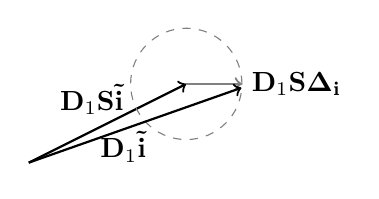
\begin{tikzpicture}
\draw [thick, ->] (0,0) -- (2,1);
\node at (0.8,0.8) {$\mathbf{D}_1\mathbf{S}\mathbf{\tilde{i}}$};
\draw [gray, thick, ->] (2,1) -- (2.707,1);
\node at (3.4,1) {$\mathbf{D}_1\mathbf{S}\mathbf{\Delta_i}$};
\draw [gray, dashed] (2,1) circle [radius=0.707];
\draw [thick, ->] (0,0) -- (2.7,0.95);
\node at (1.2,0.2) {$\mathbf{D}_1\mathbf{\tilde{i}}$};
   \end{tikzpicture}
    \caption{Vector diagram representing Eq.~\eqref{eqn:D1_smoothed}.}
    \label{fig:vec_sum}
\end{figure}



For some applications, it may be desirable to test the hypothesis of whether the intrinsic structure in a signal ${\mathbf{i}_1}$ is significantly greater than that in another signal ${\mathbf{i}_2}$. This test asks whether or not the measured difference in structure,
%
\begin{eqnarray}
\norm{\mathbf{D}_1\mathbf{S} {\mathbf{i}_1}} - \norm{\mathbf{D}_1\mathbf{S} {\mathbf{i}_2}}, \label{eqn:rel_structure}
\end{eqnarray}
%
is significant compared to \DIFdelbegin \DIFdel{the relative noise,
%DIF < 
}\begin{eqnarray*}
\DIFdel{\norm{\mathbf{D}_1\mathbf{S} \mathbf{\Delta}_{\mathbf{i}_1} - \mathbf{D}_1\mathbf{S} \mathbf{\Delta}_{\mathbf{i}_2} } = \norm{\mathbf{D}_1\mathbf{S}\left( \mathbf{\Delta}_{\mathbf{i}_1} - \mathbf{\Delta}_{\mathbf{i}_2} \right) }. \label{eqn:rel_dmerror}
}\end{eqnarray*}%DIFAUXCMD
%DIF < 
\DIFdel{Continuing the analogy of Fig. ~\ref{fig:vec_sum}, }\DIFdelend \DIFaddbegin \DIFadd{its noise. By }\DIFaddend Eq.~\DIFdelbegin \DIFdel{\eqref{eqn:rel_dmerror} represents the surface of an n-dimensional sphere with magnitude given by a combination of $\mathbf{D}_1\mathbf{S} \mathbf{\Delta}_{\mathbf{i}_1}$ and $\mathbf{D}_1\mathbf{S} \mathbf{\Delta}_{\mathbf{i}_2}$. If the difference in structure between $\mathbf{i}_1$ and $\mathbf{i}_2$ given by }\DIFdelend \DIFaddbegin \DIFadd{\eqref{eqn:expand}, the noise in }\DIFaddend Eq.~\eqref{eqn:rel_structure} is \DIFdelbegin \DIFdel{less than the radius of the sphere, the structures are consistent to within noise fluctuations. Specifically, the }\DIFdelend \DIFaddbegin \DIFadd{$e_{\parallel,1}-e_{\parallel,2}=\mathbf{w}_1\mathbf{n}_1-\mathbf{w}_2\mathbf{n}_2$, with variance
%DIF > 
}\begin{eqnarray}
\DIFadd{\sigma_{12}^2=\Var(\mathbf{w}_1\mathbf{n}_1-\mathbf{w}_2\mathbf{n}_2). \label{eqn:rel_dmerror}
}\end{eqnarray}
%DIF > 
\DIFadd{The }\DIFaddend structure in $\mathbf{i}_1$ can be said to be greater than that in $\mathbf{i}_2$ when 
%
\DIFdelbegin \begin{eqnarray*}
\DIFdel{\norm{\mathbf{D}_1\mathbf{S} {\mathbf{i}_1}} }& \DIFdel{> }& \DIFdel{\norm{\mathbf{D}_1\mathbf{S} {\mathbf{i}_2}} + \norm{\mathbf{D}_1\mathbf{S}\left( \mathbf{\Delta}_{\mathbf{i}_1} - \mathbf{\Delta}_{\mathbf{i}_2} \right) }. \label{eqn:add_error}
}\end{eqnarray*}%DIFAUXCMD
\DIFdelend \DIFaddbegin \begin{eqnarray}
\DIFadd{\norm{\mathbf{D}_1\mathbf{S} {\mathbf{i}_1}} }& \DIFadd{> }& \DIFadd{\norm{\mathbf{D}_1\mathbf{S} {\mathbf{i}_2}} + z\,\sigma_{12}. \label{eqn:add_error}
}\end{eqnarray}\DIFaddend 
\DIFaddbegin \DIFadd{Using $\norm{\mathbf{D}_1\mathbf{S}( \mathbf{\Delta}_{\mathbf{i}_1} - \mathbf{\Delta}_{\mathbf{i}_2})}$ in place of $\sigma_{12}$ is again a radius, and it contains the deterministic burst difference $\mathbf{D}_1\mathbf{S}[(\mathbf{s}_1-\mathbf{S}\mathbf{s}_1)-(\mathbf{s}_2-\mathbf{S}\mathbf{s}_2)]$, which grows away from the peak.
}\DIFaddend 


Such a test will become relevant when assessing whether the structure at one DM is significantly different from the structure at another, since \DIFdelbegin \DIFdel{$\mathbf{\Delta}_{\mathbf{i}_1}$ and $\mathbf{\Delta}_{\mathbf{i}_2}$ will in this case be correlated}\DIFdelend \DIFaddbegin \DIFadd{$\mathbf{n}_1$ and $\mathbf{n}_2$ are then the same channel noise with different delays. Near the peak $e_{\parallel,1}-e_{\parallel,2}\simeq e_\parallel'\,(d_1-d_2)$ (Appendix~B)}\DIFaddend .

\subsection{Example smoothing matrix based on discrete cosine}\label{sec:smooth_DCT}
We can choose the eigenvectors of $\mathbf{D}_1^T\mathbf{D}_1$ as the basis for the smoothing operation. As we will show later, the close connection to the first derivative $\mathbf{D}_1$ matrix lends itself to insight when expressing the entire calculation as a single matrix operation. The eigenvectors of
\begin{eqnarray}
\mathbf{D}_1^T\mathbf{D}_1=
\left[ \begin{array}{c c c c c} 
-1 & ~1 &  &  & \\ 
-1 & ~2 & -1 &  &\\
 & . & . & . & \\
 & & -1 & 2 & -1 \\
 &   &   & -1 & ~~1 
\end{array} \right],
\label{eqn:D1TD1}
\end{eqnarray} 
are discrete cosines~\citep{Strang_DCT}. We shall call this eigenvector matrix $\mathbf{C}$ whose components are
\begin{eqnarray}
\mathbf{c}_k(j)=\cos\left(j-\frac{1}{2}\right)\frac{(k-1)\pi}{N},
\label{eqn:evec_DCT2}
\end{eqnarray} 
where $k=1,\cdots,N$ is the column number of $\mathbf{C}$ and $j=1,\cdots,N$ is the row number. The eigenvalues are
\begin{eqnarray}
\text{eig}_k=2-2\cos\frac{(k-1)\pi}{N}.
\label{eqn:eval_DCT2}
\end{eqnarray}
This is known as the discrete cosine transform-2 (DCT-2). Most importantly, DCT-2 has a fast implementation based on the fast Fourier transform (FFT)~\citep{Strang_DCT}. Therefore, numerical linear algebra eigendecomposition is not needed to obtain Eq.~\eqref{eqn:evec_DCT2} and Eq.~\eqref{eqn:eval_DCT2}. 

The smoothing operation may be written as 
\begin{eqnarray}
\tilde{\mathbf{i}}=\mathbf{C}\mathbf{D}_{\rm filter}\mathbf{C}^T\mathbf{i}=\mathbf{S}\mathbf{i}, 
\label{eqn:smooth_DCT}
\end{eqnarray}
where $\mathbf{D}_{\rm filter}$ is a diagonal matrix representing a low-pass filter in the spectral domain; $\mathbf{C}^T\mathbf{i}$ is the DCT of $\mathbf{i}$ and  $\mathbf{C}(\mathbf{D}_{\rm filter}\mathbf{C}^T\mathbf{i})$ is the inverse DCT of the filtered spectrum. The diagonal of $\mathbf{D}_{\rm filter}$ is the spectral response of a low-pass filter, for example, 
\begin{eqnarray}
f(k)=\frac{1}{1+\left(\frac{k}{k_c}\right)^{2O}},
\label{eqn:butterworth}
\end{eqnarray}
where $k_c$ is the spectral cutoff and $O$ is the order of the filter. The resulting pass band is flat and the roll off rate is $2O$ orders of magnitude per decade, as inspired by the analog Butterworth filter. The DCT is purely real and does not force a periodic boundary condition (as in the case of FFT) that could introduce a discontinuity corresponding to high-frequency contents~\citep[see Ch.~8]{Strang_wavelet}.

Using smoothing process based on the DCT in Eq.~\eqref{eqn:smooth_DCT}, we can write
\begin{eqnarray}
\norm{\mathbf{D}_1\tilde{\mathbf{i}}}^2
&=&\mathbf{i}^T \mathbf{C}\mathbf{D}_{\rm filter}\mathbf{C}^T\mathbf{D}_1^T\mathbf{D}_1\mathbf{C}\mathbf{D}_{\rm filter}\mathbf{C}^T\mathbf{i} \nonumber \\
&=&\mathbf{i}^T\mathbf{C}\mathbf{D}_{\rm filter}\mathbf{\Lambda}_{D_1^TD_1}\mathbf{D}_{\rm filter}\mathbf{C}^T\mathbf{i} \nonumber\\
&=&\norm{\mathbf{\Lambda}_{D_1^TD_1}^{1/2}\mathbf{D}_{\rm filter}\mathbf{C}^T\mathbf{i}}^2
\label{eqn:sum_d1_smooth_DCT}
\end{eqnarray}
where we used the eigendecomposition $\mathbf{D}_1^T\mathbf{D}_1=\mathbf{C}\mathbf{\Lambda}_{D_1^TD_1}\mathbf{C}^T$ and $\mathbf{\Lambda}_{D_1^TD_1}$ is a diagonal matrix of non-negative eigenvalues, $\text{eig}_k$, shown in Eq.~\eqref{eqn:eval_DCT2}; $\mathbf{C}^T\mathbf{C}=\mathbf{I}$ since $\mathbf{C}$ is an orthogonal matrix. Eq.~\eqref{eqn:sum_d1_smooth_DCT} is a key result. It expresses the final product which is the sum of the square of the derivative of the smoothed data in terms of the end-to-end matrix operation. We note that $\mathbf{\Lambda}_{D_1^TD_1}^{1/2}$ is a diagonal matrix whose diagonal represents a high pass profile such that $\mathbf{\Lambda}_{D_1^TD_1}^{1/2}\mathbf{D}_{\rm filter}$ represents a band pass filter with the peak response at approximately $k_c$ as shown in Fig.~\ref{fig:filter_resp}. The norm (subscript $._2$ is not shown for brevity)  of the smoothed data is the structure parameter, $\sqrt{\Sigma(d/dt)^2}$,
\begin{eqnarray}
\norm{\mathbf{D}_1\tilde{\mathbf{i}}}=\norm{\mathbf{\Lambda}_{D_1^TD_1}^{1/2}\mathbf{D}_{\rm filter}\mathbf{C}^T\left(\tilde{\mathbf{i}}+\mathbf{\Delta_i}\right)}. 
\label{eqn:norm_res}
\end{eqnarray} 
Finally, the \DIFdelbegin \DIFdel{uncertainty }\DIFdelend \DIFaddbegin \DIFadd{residual length of Eq.~\eqref{eqn:norm_D1Si} }\DIFaddend is 
\begin{eqnarray}
\norm{\mathbf{D}_1\mathbf{S}\mathbf{\Delta}_\mathbf{i}}=\norm{\mathbf{\Lambda}_{D_1^TD_1}^{1/2}\mathbf{D}_{\rm filter}\mathbf{C}^T\mathbf{\Delta_i}}.
\label{eqn:norm_del}
\end{eqnarray}
Expressing the 2-norm in the spectral domain as we have done above has an advantage in visualization. For example, $\mathbf{C}^T\mathbf{i}$ is the spectrum of $I(t)$. Pre-multiplying that quantity by $\mathbf{\Lambda}_{D_1^TD_1}^{1/2}\mathbf{D}_{\rm filter}$ filters the spectrum. Finally, taking the norm measures the length of the resulting vector.

\DIFaddbegin \DIFadd{In practice $\hat{\mathbf{a}}$ is estimated from the data, $\hat{\mathbf{a}}\simeq\mathbf{D}_1\mathbf{S}\mathbf{i}/\norm{\mathbf{D}_1\mathbf{S}\mathbf{i}}$, and $\mathbf{w}=\hat{\mathbf{a}}^T\mathbf{D}_1\mathbf{S}$ is obtained by differencing $\hat{\mathbf{a}}$ and smoothing the result with $\mathbf{S}$. The noise level is measured from the same on-pulse spectrum in the band $k>N/4$, where the burst has no power,
}\begin{eqnarray}
\DIFadd{\hat\sigma_n=1.4826\,{\rm median}_{k>N/4}|(\mathbf{C}^T\mathbf{i})_k|,
\label{eqn:sigma_DCT}
}\end{eqnarray}
\DIFadd{since the orthonormal DCT (columns of $\mathbf{C}$ normalised) leaves the white-noise variance unchanged in every mode. Then $\sigma^2=\hat\sigma_n^2\sum_tw_t^2$. For self-noise, $\sigma^2=\sum_tw_t^2\sigma_t^2$, with $\sigma_t^2$ the local mean square of the series rebuilt from the modes $k>N/4$, divided by $3/4$.
}

\DIFaddend \begin{figure}[htb]
\begin{center}
\noindent
  \includegraphics[width=2.5in]{figs/Bandpass_responnse.pdf}
\caption{$\mathbf{\Lambda}_{D_1^TD_1}^{1/2}\mathbf{D}_{\rm filter}$ band pass filter response for $k_c=4, 15, 100$ for an $O=3$ filter defined by Eq.~\eqref{eqn:butterworth}.}
\label{fig:filter_resp}
\end{center}
\end{figure}


\section{Result: Numerical Example} \label{sec:result}

\subsection{Selection of Filter Parameters} \label{sec:numex_filt}
We exemplify the method discussed in  \secref{sec:unc_def} by demonstrating the selection of filter parameters to correctly recover the underlying $I(t)$ structure in the presence of noise. Fig.~\ref{fig:I_and_spec} (top) shows 1000 noisy $I=|X|^2+|Y|^2$ data points with an underlying double pulse as shown, representing total power $I$ calculated from perpendicular $X$ and $Y$ linearly polarized voltage components. The noise-free component of $X$ consists of two Gaussian pulses delayed by 370 and 630 units with standard deviations of 80 and 85, respectively. The amplitude is normalized to the pulse peak. The noise-free amplitude of the $Y$ component is taken as $0.5X$. The structure parameter of the noise-free pulse is $\norm{\mathbf{D}_1\mathbf{i}_{\text{noiseless}}}=0.18$ as computed by the 2-norm of the first derivative. The noise in the complex voltages $X,~Y$ are independent and identically distributed Gaussian noise with zero mean and standard deviation $\sigma_{\Re(X)}=\sigma_{\Im(X)}=\sigma_{\Re(Y)}=\sigma_{\Im(Y)}=0.4$. The DCT spectrum of the signal is depicted in Fig.~\ref{fig:I_and_spec} (bottom). It shows that the information occupies up to a $k$ index of 10 to 20, beyond which the noise dominates.  Therefore, we expect to select a low-pass filter cutoff between $k_c$ of 10 to 20. 

\begin{figure}[htb]
\begin{center}
\noindent
  \includegraphics[width=3.25in]{figs/Fig3_update.pdf}
\caption{Example noisy pulse (top) and the corresponding spectrum in discrete cosine (bottom). The underlying pulse consists of two unity amplitude Gaussians. The solid black curve in the top plot represents the recovered intensity with filter parameters $O=3,~k_c=15$.}
\label{fig:I_and_spec}
\end{center}
\end{figure}

The $k_c$ estimate based on the DCT spectrum is confirmed by the calculated structure parameter and the uncertainty shown in Fig.~\ref{fig:unc_filter} where the low-pass filter cutoff $k_c$ was swept from 3 to 300 for filter order 2, 3, 4 in Eq.~\eqref{eqn:butterworth} to explore the effects of under- and over-filtering.  The structure parameter was computed using Eq.~\eqref{eqn:norm_res} and the associated uncertainty was calculated using \DIFaddbegin \DIFadd{the original radius $\norm{\mathbf{D}_1\mathbf{S}\mathbf{\Delta_i}}/\norm{\mathbf{D}_1\mathbf{S}\tilde{\mathbf{i}}}$. With }\DIFaddend Eq.~\eqref{eqn:rel_error} \DIFaddbegin \DIFadd{the uncertainties in Fig.~\ref{fig:unc_filter} are lower by the square root of Eq.~\eqref{eqn:ratio}, and their $k_c$ dependence needs recomputing}\DIFaddend . The structure parameter obtained from the smoothed noisy data matches the known noise-free value of 0.18 for $k_c$ between 10 to 20, which agrees with that suggested by the DCT spectrum. This also coincides with the range of $k_c$ values for which the uncertainty is minimized. We also note that the structure parameter becomes rapidly underestimated and overestimated as the $k_c$ is underestimated (over-smoothing) and overestimated (under-smoothing), respectively. The uncertainty minima at $k_c$ of approximately 5 for filter orders 3 and 4 in Fig.~\ref{fig:unc_filter} correspond to over-smoothing which may be readily identified from the DCT spectrum in Fig.~\ref{fig:I_and_spec} and confirmed by the recovered structure parameter. Proper determination of $k_c$ is therefore critical, and we demonstrate that the DCT spectrum is a very effective tool for that purpose.

\begin{figure}[htb]
\begin{center}
\noindent
  \includegraphics[width=3.25in]{figs/Simulation_dbl_pulse_struct_unc_31mar2022_for_paper.pdf}
\caption{Recovered structure parameter (top) and uncertainty (bottom) of the structure parameter for $k_c$ swept from 3 to 300 and filter order 2, 3, 4 in Eq.~\eqref{eqn:butterworth}.}
\label{fig:unc_filter}
\end{center}
\end{figure}

\subsection{Robustness with respect to $\Delta$\,DM} \label{sec:numex_DM}

The previous sub-section operated on one-dimensional time-series data, which assumes that de-dispersion has already been performed.  However, in reality, the dispersion measure is not known a priori (otherwise the problem would already be solved!) and hence it is necessary to consider whether de-dispersing across different trial DM values could affect the parameter choice and hence final results. In this sub-section, we simulate the effects of dispersion and de-dispersion on the double pulse already considered.

In the frequency domain, the net effect of dispersion and de-dispersion may be described as a multiplicative factor
%
\begin{eqnarray}
e^{-j(k(\nu)-\tilde{k}(\nu))L} = e^{-j(2\pi)K_{\rm DM}\frac{-\Delta\text{DM}\text[\pccc]}{\nu[\text{MHz}]}}. 
\label{eqn:disp-dedisp}
\end{eqnarray}
The units in Eq.~\eqref{eqn:disp-dedisp} follow the convention described in~\citet{Wilson2009}; $L$ is the distance to the source and $k(\nu)$ and $\tilde{k}(\nu)$ are the wavenumber and the wavenumber estimate, respectively; the difference between the actual DM and the DM estimate is $\Delta\text{DM}=\text{DM}-\tilde{\text{DM}}$.
Throughout, we define the delay constant $K_{\rm DM}$ to be $(1/0.241) \cdot 10^9 \approx 4.149 \cdot 10^9$\,MHz\,cm$^{3}$\,pc$^{-1}$.
Hence, the effects of dispersion and de-dispersion may be simulated by multiplying Eq.~\eqref{eqn:disp-dedisp} with the Fourier transform (FT) of the noisy complex voltages, followed by inverse FT of the product.

As an example, we took a $256\times1024$ matrix of complex white noise with $\sigma_{\rm re}=\sigma_{\rm im}=1/\sqrt{2}$. This noise matrix was multiplied by two 2-D Gaussian real envelopes, then complex Gaussian noise with $\sigma_{\rm re}=\sigma_{\rm im}=1/2\sqrt{2}$ was added. The result shown in Fig.~\ref{fig:FT_DM0} is the simulated data at $\Delta\text{DM}=0$. We chose the time delays between the components to mimic the `sad trombone' effect, i.e.\ the frequency down-drift of burst components with time, often seen in repeating FRBs \citep[e.g.][]{Hessels_2019}.

\begin{figure}[htb]
\begin{center}
  \includegraphics[width=3.25in]{figs/Fig5_2Feb2023.pdf}
\caption{The frequency-time simulated frequency down-drifting data at $\Delta\text{DM}=0$ (top). The bottom figure shows the mean intensity over frequency of the noisy data (solid line) and the Gaussian envelope (dashed line).}
\label{fig:FT_DM0}
\end{center}
\end{figure}

We applied $\Delta\text{DM}$ from $-0.5$ to $0.2\, \text{pc} \,\text{cm}^{-3}$ in $0.01\,\text{pc}\, \text{cm}^{-3}$ steps. The resulting noisy mean intensities vs.\ time over $\Delta\text{DM}$ are shown in Fig.~\ref{fig:I_DM_noF}. The intensity of the noise-free data was simulated by applying the corresponding group delay $\tau_d=4.149\times10^3\Delta \text{DM} [\text{pc} \, \text{cm}^{-3}]/f_{\rm MHz}^2$ to the intensity envelope. To filter the noise in Fig.~\ref{fig:I_DM_noF}, we applied the same strategy discussed in \secref{sec:numex_filt}. We performed DCT of the frequency-time  $256\times1024$ data shown Fig.~\ref{fig:FT_DM0} and then visually inspected the resulting DCT spectrum (not shown). The transition between information and noise occurred at $k$ index of approximately 35. Therefore, we set $k_c=35$ and $O=3$ was kept the same as the previous section.

\begin{figure}[htb]
\begin{center}
  \includegraphics[width=3.25in]{figs/Fig6_2Feb2023.pdf}
\caption{Intensities vs.\ time and $\Delta \text{DM}$ of simulated frequency down-drifting data before filtering.}
\label{fig:I_DM_noF}
\end{center}
\end{figure}

Fig.~\ref{fig:Stuct_DM}  summarizes the robustness of the method we propose in this paper with respect to $\Delta\text{DM}$. Fig.~\ref{fig:Stuct_DM} (top) shows the comparison between the recovered (from the noisy data) and the known structure parameters (from the noise-free intensity envelope that was time shifted as per the group delay at each frequency).
The difference between the two are plotted in the second row. The uncertainty computed using \DIFdelbegin \DIFdel{Eq.~\eqref{eqn:rel_error} }\DIFdelend \DIFaddbegin \DIFadd{the original radius }\DIFaddend is shown in the third row \DIFaddbegin \DIFadd{(needs recomputing with Eq.~\eqref{eqn:rel_error})}\DIFaddend . Finally, the maximum recovered intensity is shown at the bottom of  Fig.~\ref{fig:Stuct_DM}. From this figure, we infer the following. The filter recovers the correct structure parameters to within a few percent for all trial $\Delta\text{DM}$s. The recovered highest structure parameter at $\Delta\text{DM}\approx 0$ and the maximum intensity at $\Delta\text{DM}\approx -0.26$\,\pccc\ are consistent with the noise-free intensity envelope. For the selected filter, the uncertainty of $\sim5$\% to 10\% in the measured structure is comparable across $\Delta\text{DM}$s. At $\Delta\text{DM}=0$, where the structure is maximised but the intensity is lower than the highest peak, the uncertainty appears slightly lower.

To derive an uncertainty in $\Delta \text{DM}$, we take the noise estimates $\Delta_{\mathbf{i}}$ at the structure-maximised value $\Delta$DM=0, and subtract the noise estimates at other values of $\Delta$DM. This \DIFaddbegin \DIFadd{difference also contains the burst residual difference, which is not noise. This }\DIFaddend is shown in Figure~\ref{fig:relative_noise_example}. The magnitude of the relative errors\DIFdelbegin \DIFdel{as per }\DIFdelend \DIFaddbegin \DIFadd{, from the original radius form of }\DIFaddend Eq.~\eqref{eqn:rel_dmerror} \DIFaddbegin \DIFadd{(needs recomputing), }\DIFaddend are given in Fig.~\ref{fig:Stuct_DM}. For values of $\Delta$DM near $0$, the relative uncertainty (dashed line in third panel from top) is smaller than the absolute uncertainty (solid line) due to strong correlations in the filtered noise. At large values of $\Delta$DM however, the noise becomes uncorrelated, and so is approximately $\sqrt{2}$ times the absolute value.


\begin{figure*}
\centering
  \includegraphics[width=6in]{figs/Fig8_2Feb2023.pdf}
\caption{Calculated structure parameter (top), difference between the structure parameter of the recovered signal and the original time-delayed envelope (second row), uncertainty of the recovered structure parameter (third row), maximum recovered intensity (bottom), of simulated frequency down-drift data.
}
\label{fig:Stuct_DM}
\end{figure*}

\begin{figure}
    \centering
    \includegraphics[width=3.25in]{figs/Fig7_2Feb2023.pdf}
    \caption{The vector $\mathbf{D}_1\mathbf{S}\left( \mathbf{\Delta}_{\Delta {\rm DM}=0} - \mathbf{\Delta}_{\Delta {\rm DM}} \right)$ \DIFdelbeginFL \DIFdelFL{from }\DIFdelendFL \DIFaddbeginFL \DIFaddFL{used in the original radius form of }\DIFaddendFL Eq.~\eqref{eqn:rel_dmerror}, calculated for simulated frequency down-drifting data. }
    \label{fig:relative_noise_example}
\end{figure}

\DIFdelbegin \DIFdel{To derive error bounds for $\Delta$DM , we add the error to the structure as per the right-hand-side }\DIFdelend \DIFaddbegin \DIFadd{The DM uncertainty is the scatter of the structure peak, $\sigma_{\rm DM}$ }\DIFaddend of Eq.~\DIFdelbegin \DIFdel{\eqref{eqn:add_error}, also shown in Fig.~\ref{fig:Stuct_DM}. The uncertainty in $\Delta$DM corresponds to those regions where the relative noise plus the intrinsic structure exceeds that of the structure at $\Delta$DM$=0$, i.e.\ which can not be excluded by Eq.~(\eqref{eqn:add_error}). Thus we find $\Delta$DM$=0_{-0.04}^{+0.08}$\,}%DIFDELCMD < \pccc%%%
\DIFdelend \DIFaddbegin \DIFadd{\eqref{eqn:sigma_DM}. If an interval test such as Eq.~\eqref{eqn:add_error} is used instead, the region where $\norm{\mathbf{D}_1\mathbf{S}\mathbf{i}_{\hat d}}-\norm{\mathbf{D}_1\mathbf{S}\mathbf{i}_d}\le z\,\sigma_{12}$ has half-width $2z\,\sigma_{\rm DM}$, so $z=\tfrac12$ gives $1\sigma$ (Appendix~B). The original value here, from the radius with $z=1$, needs recomputing; in our simulations that procedure overestimates $\sigma_{\rm DM}$ by a factor of 9--13}\DIFaddend .


\section{Result: Application to FRB data} \label{sec:apply}

The above methods can be applied to determine the correct DM of an FRB, and the uncertainty thereon. Dedispersing an FRB for many trial DMs produces voltage time series that can be converted into intensity time-series $\mathbf{i}$. The procedure of Sec.~\secref{sec:method} then produces a corresponding measure of FRB structure and its uncertainty for each and every trial DM. This then allows the trial DM that maximizes structure to be identified, and an error in DM assigned to include the range of trial DMs with structure consistent with the maximum value, given the calculated structure error.

\subsection{FRB181112} \label{sec:181112}
We apply our method to FRB181112~\citep{cho_2020ApJ...891L..38C} data averaged to 1\,$\mu$s. Fig.~\ref{fig:FRB_DM_t} shows the raw intensity data as a function of dispersion measure, away from the nominal value of 589.265\,pc\,cm$^{-3}$ that produces the maximum signal to noise (S/N) ratio. The spectrum of the intensity time series was obtained by the multiplication with the discrete cosine matrix discussed in Sec.~\ref{sec:smooth_DCT}. This is shown in Fig.~\ref{fig:FRB_spec}. We observe that the information occupies up to $k=30$ index, after which it is dominated by noise. Based on this information, we selected the filter cutoff of $k_c=30$ and chose a $O=3$ filter as per Eq.~\eqref{eqn:butterworth}.

\begin{figure}[htb]
\begin{center}
\noindent
    \includegraphics[width=3.0in]{figs/Fig8_refresh.pdf}
\caption{Intensity of FRB181112 vs.\ time and $\Delta$ DM in pc\,cm$^{-3}$ from the DM that produces maximum S/N.}
\label{fig:FRB_DM_t}
\end{center}
\end{figure}

\begin{figure}[htb]
\begin{center}
\noindent
  \includegraphics[width=2.75in]{figs/FRB181112_spectrum.pdf}
\caption{Spectrum of FRB~181112 in discrete cosine domain shown in absolute values for all $\Delta$DM.}
\label{fig:FRB_spec}
\end{center}
\end{figure}


The first derivative of the smoothed data is reported in Fig.~\ref{fig:FRB_D1_smooth}. Finally, the structure parameter and the corresponding uncertainty are plotted in Fig.~\ref{fig:FRB_struc}. We see that the highest structure coincides with $\Delta$DM=0 which is the maximum S/N. The uncertainty has a trend that increases away from $\Delta {\rm DM}=0$, while the relative uncertainty compared to $\Delta{\rm DM}=0$ increases even more strongly. We find that allowing the structure to fluctuate upwards by one standard deviation of relative noise allows structure within $\Delta{\rm DM} = 0 \pm 0.011$\,\pccc\ to exceed the peak value of $12.2\times10^{-5}$ at $\Delta {\rm DM}=0$, i.e.\ our uncertainty in $\Delta {\rm DM}$ is $0.011$\,\pccc. \DIFaddbegin \DIFadd{This value used the original radius and needs recomputing with Eq.~\eqref{eqn:sigma_DM}.
}\DIFaddend 

\begin{figure}[htb]
\begin{center}
\noindent
  \includegraphics[width=3.0in]{figs/Fig10_refresh.pdf}
\caption{First derivative of the intensity of FRB181112 vs.\ time and $\Delta$DM after smoothing using $k_c=30$ and $O=3$ filter.}
\label{fig:FRB_D1_smooth}
\end{center}
\end{figure}

\begin{figure}[htb]
\begin{center}
\noindent
  \includegraphics[width=3.25in]{figs/Fig12_clancy.pdf}
\caption{Solid lines: Structure parameter of FRB181112 computed using $\sqrt{\Sigma(d/dt)^2}$ ($k_c=30, O=3$) (top), and the corresponding uncertainty (bottom). Dashed lines: \DIFdelbeginFL \DIFdelFL{68\% }\DIFdelendFL upper limits \DIFaddbeginFL \DIFaddFL{from the original radius test (not 68\%; Sect.~\ref{sec:numex_DM}) }\DIFaddendFL on structure (top), and relative error (bottom), with respect to $\Delta$DM$=0$\,\pccc.}
\label{fig:FRB_struc}
\end{center}
\end{figure}

\subsection{FRB210117} \label{sec:210117}
Next, we consider FRB210117 with time-domain data at 10\,$\mu$s resolution shown in Fig.~\ref{fig:FRB210117_Raw} for the indicated $\Delta$DM, relative to the nominal S/N maximizing value of 729.2\,pc\,cm$^{-3}$ \citep{Bhandari2022}. This FRB appears to have a secondary peak for $\Delta\text{DM}<0$. The spectrum of this FRB (not shown) suggests a spectral transition at a $k$ value between 25 and 35. This is shown in Fig.~\ref{fig:FRB210117_kc_bounds} where we plot the best-fitting $\Delta$DM and \DIFdelbegin \DIFdel{68\% }\DIFdelend uncertainty bounds as per \DIFaddbegin \DIFadd{the original radius form of }\DIFaddend Eq.~\eqref{eqn:add_error} \DIFaddbegin \DIFadd{(not 68\%) }\DIFaddend over filter cutoff $k_c$ (with $O=3$). It shows that $k_c\approx$25--35 offers consistent values of the structure-maximising $\Delta$DM with the narrowest error margin. Using lower values of $k_c$ results in over-smoothing, and thus a loss of signal structure; while using higher values of $k_c$ adds noise, increasing the random error in $\Delta$DM.

\begin{figure}[tb]
\begin{center}
\noindent
  \includegraphics[width=3.0in]{figs/Fig13_refresh.pdf}
\caption{Intensity before smoothing of FRB210117 vs.\ time and $\Delta$DM from the DM that produces maximum S/N.}
\label{fig:FRB210117_Raw}
\end{center}
\end{figure}

The structure parameter and the associated uncertainty are plotted in Fig.~\ref{fig:FRB210117_struc_unc}. Using the same procedure as for FRB~20181112, we find a structure-maximising $\Delta\text{DM}=-0.1_{-0.23}^{+0.36}$\,\pccc\DIFaddbegin \DIFadd{\ (uncertainty to be recomputed with Eq.~\eqref{eqn:sigma_DM})}\DIFaddend . Thus, we cannot exclude that this FRB's apparent structure-maximising DM is significantly different from its signal-to-noise maximising DM.

\begin{figure}[tb]
\begin{center}
\noindent
\includegraphics[width=3.0in]{figs/210117_kc_var_uncertainty.png}
\caption{Structure maximising $\Delta$DM (solid) and \DIFdelbeginFL \DIFdelFL{68\% }\DIFdelendFL error bounds \DIFaddbeginFL \DIFaddFL{from the original radius test }\DIFaddendFL (dashed\DIFaddbeginFL \DIFaddFL{; not 68\%}\DIFaddendFL ) for FRB210117 as a function of filter cutoff $k_c$ ($O=3$).}
\label{fig:FRB210117_kc_bounds}
\end{center}
\end{figure}

\begin{figure}[tb]
\begin{center}
\noindent
  \includegraphics[width=3.25in]{figs/Fig15_Feb2023.pdf}
\caption{Solid lines: Structure parameter of FRB210117 (top) and the corresponding uncertainty with $k_c=27$ and $O=3$ smoothing filter (bottom). Dashed lines: \DIFdelbeginFL \DIFdelFL{68\% }\DIFdelendFL upper limit \DIFaddbeginFL \DIFaddFL{from the original radius test (not 68\%; Sect.~\ref{sec:numex_DM}) }\DIFaddendFL on structure (top), and relative uncertainty (bottom), with respect to $\Delta$DM$=-0.2$\,\pccc.}
\label{fig:FRB210117_struc_unc}
\end{center}
\end{figure}


\section{Conclusion} \label{sec:concl}
We demonstrated that computing the structure parameter using the 2-norm, $\sqrt{\Sigma (d/dt)^2}$, permits a direct calculation of the uncertainty of the resulting structure parameter. The uncertainty \DIFdelbegin \DIFdel{of the first derivative of the smoothed data is calculated by taking the difference between the structure parameter of the smoothed data and the structure parameter of the }\DIFdelend \DIFaddbegin \DIFadd{is the scatter of the noise projected onto the structure direction, Eq.~\eqref{eqn:sigma}. The length of the residual between the smoothed and }\DIFaddend ``double-smoothed\DIFdelbegin \DIFdel{" data. The latter can be obtained easily by taking the smoothed data (before taking the derivative) and plugging it back as the input to the algorithm}\DIFdelend \DIFaddbegin \DIFadd{'' data overestimates it by the square root of Eq.~\eqref{eqn:ratio}, a factor of 5--9 in our simulations}\DIFaddend . We have also shown how to use this uncertainty for statistical tests for different intrinsic structure between two filtered signals.

This method was applied to FRB181112 and  FRB210117. In the case of FRB181112, the DM that produces the highest S/N is the same as that with the highest structure within an uncertainty in $\Delta$DM of $\pm0.011$\,\pccc. As for FRB210117, the highest structure occurred at a  $\text{DM}=729.1_{-0.23}^{+0.36}$\,\pccc, compared to the signal-to-noise maximising DM of $729.2$\,\pccc. \DIFaddbegin \DIFadd{Both DM uncertainties need recomputing with Eq.~\eqref{eqn:sigma_DM}.
}\DIFaddend 


\begin{acknowledgments}
The Australian SKA Pathfinder is part of the Australia Telescope National Facility (https://ror.org/05qajvd42) which is managed by CSIRO. Operation of ASKAP is funded by the Australian Government with support from the National Collaborative Research Infrastructure Strategy. ASKAP uses the resources of the Pawsey Supercomputing Centre. Establishment of ASKAP, the Murchison Radio-astronomy Observatory and the Pawsey Supercomputing Centre are initiatives of the Australian Government, with support from the Government of Western Australia and the Science and Industry Endowment Fund. We acknowledge the Wajarri Yamatji people as the traditional owners of the Observatory site.
CWJ and MG acknowledge support from the Australian Government through the Australian Research Council's Discovery Projects funding scheme (project DP210102103). This work made use of \textsc{Scipy} \citep{SciPy2019}.
\end{acknowledgments}

\section*{Appendix} \label{sec:app}
We now briefly discuss other definitions of structure parameters: $\Sigma \left(d/dt\right)^2$~\citep{Hessels_2019}, $\Sigma \left|d/dt\right|$~\citep{Gajjar_2018}, and $\Sigma \left(d/dt\right)^4$~\citep{Josephy_2019}. We note that $\Sigma \left|d/dt\right|$ is the 1-norm of the vector derivative of the smoothed data~\citep[see Ch.~1]{Strang_LALD2019}. This means the triangle inequality is fulfilled, $\norm{\mathbf{x}+\mathbf{y}}_1\leq\norm{\mathbf{x}}_1+\norm{\mathbf{y}}_1$ and the upper bound is defined. However, the inner product is not defined in the 1-norm~\citep[see. Ch.~1]{Strang_LALD2019}. As a result, the corresponding lower bound cannot be shown to be that in Eq.~\eqref{eqn:D1_norm} for the 2-norm case\footnote{One can use the reverse triangle inequality to show $\norm{\mathbf{x}-\mathbf{y}}_1\geq\left|\norm{\mathbf{x}}_1-\norm{\mathbf{y}}_1\right|$, but this not the same as establishing the lower bound of $\norm{\mathbf{x}+\mathbf{y}}_1$.}. Furthermore, we are not able to relate the standard deviation estimate, such as Eq.~\eqref{eqn:norm_D1Si} in the 2-norm, to a corresponding statistical quantity in the 1-norm.

$\Sigma \left(d/dt\right)^2$ and $\Sigma \left(d/dt\right)^4$ do not conform to the norm definition because they are missing $\sqrt{}$ and $\sqrt[4]{}$ operators which would have made them 2-norm and 4-norm, respectively~\citep[see Ch.~7]{Laub_LA}. Therefore for these definitions, the triangle inequality does not apply and we are not able to establish the bounds of the summation of two vectors.

In \citet{Gajjar_2018}, the uncertainty of the structure parameter was inferred from the off-pulse system noise. This assumes that the noise during the FRB pulse is the same that of the system noise. However, it is entirely possible that the FRB pulse is noise-like and hence the on-pulse noise is different from the off-pulse noise. In fact, the noise statistics of the FRB is in itself an interesting subject for study, and therefore, it is desirable that the uncertainty be inferred from that same on-pulse data\DIFaddbegin \DIFadd{. Measuring $\sigma_n$ from the $k>N/4$ band of the on-pulse spectrum (Eq.~\ref{eqn:sigma_DCT}) does this.
}

\section*{\DIFadd{Appendix B: Corrected uncertainty}} \label{sec:appB}
\textit{\DIFadd{Expansion.}} \DIFadd{With $\mathbf{a}$, $\mathbf{e}$, $\hat{\mathbf{a}}$, $e_\parallel$ and $\mathbf{e}_\perp$ as in }\secref{sec:unc_def}\DIFadd{, Pythagoras gives $\norm{\mathbf{D}_1\tilde{\mathbf{i}}}^2=(\norm{\mathbf{a}}+e_\parallel)^2+\norm{\mathbf{e}_\perp}^2$. For $\norm{\mathbf{e}_\perp}\ll\norm{\mathbf{a}}$, $\sqrt{X^2+Y^2}\simeq X+Y^2/2X$ gives Eq.~\eqref{eqn:expand} to second order in the noise.
}

\textit{\DIFadd{Variance.}} \DIFadd{$\norm{\mathbf{a}}$ is fixed and the last term of Eq.~\eqref{eqn:expand} is second order, so to first order the variance of the structure parameter is that of $e_\parallel=\mathbf{w}\mathbf{n}=\sum_tw_tn_t$. Since $\langle e_\parallel\rangle=\sum_tw_t\langle n_t\rangle=0$, $\sigma^2=\langle e_\parallel^2\rangle=\sum_t\sum_{t'}w_tw_{t'}\langle n_tn_{t'}\rangle=\mathbf{w}\,{\rm Cov}(\mathbf{n})\,\mathbf{w}^T$, which is Eq.~\eqref{eqn:sigma}. For noise uncorrelated between samples only $t'=t$ survives, $\sigma^2=\sum_tw_t^2\sigma_t^2$.
}

\textit{\DIFadd{Estimated direction.}} \DIFadd{Estimating $\hat{\mathbf{a}}$ by $\mathbf{D}_1\mathbf{S}\mathbf{i}/\norm{\mathbf{D}_1\mathbf{S}\mathbf{i}}=(\mathbf{a}+\mathbf{e})/\norm{\mathbf{a}+\mathbf{e}}$ tilts it by $\theta\simeq\norm{\mathbf{e}_\perp}/\norm{\mathbf{a}}$. For any fixed matrix $\mathbf{M}$ and noise uncorrelated between samples, $\langle\norm{\mathbf{M}\mathbf{n}}^2\rangle=\sum_j\sum_tM_{jt}^2\sigma_t^2$. With $\mathbf{M}=\mathbf{D}_1\mathbf{S}$ this gives $\langle\norm{\mathbf{e}}^2\rangle\simeq$\,40--45\,$\sigma^2$ in our simulations, and $\langle\norm{\mathbf{e}_\perp}^2\rangle=\langle\norm{\mathbf{e}}^2\rangle-\sigma^2$, so $\theta\simeq6\sigma/\norm{\mathbf{a}}$: the estimate is good when $\norm{\mathbf{a}}\gg6\sigma$.
}

\textit{\DIFadd{Bias.}} \DIFadd{$b=\langle\norm{\mathbf{D}_1\tilde{\mathbf{i}}}\rangle-\norm{\mathbf{a}}=\langle\norm{\mathbf{e}_\perp}^2\rangle/2\norm{\mathbf{a}}=(\langle\norm{\mathbf{e}}^2\rangle-\sigma^2)/2\norm{\mathbf{a}}$. It varies slowly with DM, does not move the peak at first order, and is not an uncertainty.
}

\textit{\DIFadd{What Eq.~\eqref{eqn:norm_D1Si} measures.}} \DIFadd{The cross term of $\norm{\mathbf{d}_s+\mathbf{d}_n}^2$ has zero mean, so $\langle\norm{\mathbf{D}_1\mathbf{S}\mathbf{\Delta_i}}^2\rangle=\norm{\mathbf{d}_s}^2+\langle\norm{\mathbf{d}_n}^2\rangle$, with $\langle\norm{\mathbf{d}_n}^2\rangle$ from the expression above for $\mathbf{M}=\mathbf{D}_1\mathbf{S}-\mathbf{D}_1\mathbf{S}\mathbf{S}$, since $\mathbf{d}_n=(\mathbf{D}_1\mathbf{S}-\mathbf{D}_1\mathbf{S}\mathbf{S})\mathbf{n}$. Dividing by $\sigma^2$ gives Eq.~\eqref{eqn:ratio}. Per DCT mode $k$ (Eq.~\ref{eqn:sum_d1_smooth_DCT}), $\mathbf{D}_1\mathbf{S}$ multiplies by $\text{eig}_k^{1/2}f(k)$ and $\mathbf{D}_1\mathbf{S}-\mathbf{D}_1\mathbf{S}\mathbf{S}$ by $\text{eig}_k^{1/2}f(k)[1-f(k)]$, which peaks near $k_c$, where the filter passes half. Only the residual noise near $k_c$ survives, so the first factor of Eq.~\eqref{eqn:ratio} is $\langle\norm{\mathbf{e}}^2\rangle/\sigma^2\simeq$\,40--45 reduced by $\langle\norm{\mathbf{e}}^2\rangle/\langle\norm{\mathbf{d}_n}^2\rangle\simeq7.7$, i.e.\ 5--6. $\mathbf{d}_s$ also lies near $k_c$, where the cutoff is chosen so that the burst is comparable to the noise; it is not noise, and $\norm{\mathbf{d}_s}^2/\langle\norm{\mathbf{d}_n}^2\rangle\propto({\rm S/N})^2$ at fixed $k_c$.
}

\textit{\DIFadd{DM uncertainty.}} \DIFadd{At trial DM $d$, the structure parameter is $\mathcal{S}_d=\norm{\mathbf{D}_1\tilde{\mathbf{i}}_d}\simeq\norm{\mathbf{a}(d)}+e_\parallel(d)$. Let $d_0$ be the peak of the noise-free $\norm{\mathbf{a}(d)}$. Near it, $\norm{\mathbf{a}(d)}\simeq\norm{\mathbf{a}(d_0)}+\tfrac12\norm{\mathbf{a}}''(d_0)(d-d_0)^2$ and $e_\parallel(d)\simeq e_\parallel(d_0)+e_\parallel'(d_0)(d-d_0)$: the noise value lifts the curve and the noise slope tilts it. Setting the derivative to zero at the measured peak $\hat d$ gives $\hat d-d_0=-e_\parallel'(d_0)/\norm{\mathbf{a}}''(d_0)$, so $\sigma_{\rm DM}={\rm std}[e_\parallel'(d_0)]/|\norm{\mathbf{a}}''(d_0)|$. Write $e_\parallel(d)=\sum_tw(t;d)\,n(t;d)$, with $w(t;d)$ the weight row at DM $d$ and $n(t;d)=\sum_{\nu}x_{\nu}(t+d\,\tau_{\nu})$ the dedispersed noise, where $x_{\nu}(t)$ is the noise in channel $\nu$ at sample $t$ and $\tau_{\nu}=K_{\rm DM}(\nu^{-2}-\nu_{\rm ref}^{-2})/t_{\rm samp}$ is its delay per unit DM in samples. Relabelling $t\to t-d\,\tau_{\nu}$ in each channel moves all the dependence on $d$ into the smooth weights, $e_\parallel(d)=\sum_{\nu}\sum_tw(t-d\,\tau_{\nu};d)\,x_{\nu}(t)$, so $e_\parallel'(d_0)=\sum_{\nu}\sum_tw'_{\nu}(t)\,x_{\nu}(t)$ with $w'_{\nu}(t)=\partial_d\,w(t-d\,\tau_{\nu};d)|_{d_0}$. For channel noise independent between channels and samples, with variance $\sigma_{\nu}^2$,
}\begin{eqnarray}
\DIFadd{\sigma_{\rm DM}=\frac{\big(\sum_{\nu}\sigma_{\nu}^2\sum_tw'_{\nu}(t)^2\big)^{1/2}}{|\norm{\mathbf{a}}''(d_0)|}.
\label{eqn:sigma_DM}
}\end{eqnarray}
\DIFadd{This holds for any burst morphology (drift, scattering) and does not depend on $\nu_{\rm ref}$. In practice $d_0\to\hat d$, and $w'_{\nu}$ is a central difference,
}\begin{eqnarray}
\DIFadd{w'_{\nu}(t)}&\DIFadd{\simeq}&\DIFadd{\frac{1}{2\delta}\big[w(t-(\hat d+\delta)\tau_{\nu};\hat d+\delta)\nonumber}\\
&&\DIFadd{-\,w(t-(\hat d-\delta)\tau_{\nu};\hat d-\delta)\big],\nonumber
}\end{eqnarray}
\DIFadd{with each row computed from the data dedispersed at that DM and $\delta\simeq\sigma_{\rm DM}/2$. $\norm{\mathbf{a}}''$ is the curvature of the measured structure curve: either $2c_2$ from a least-squares parabola $c_0+c_1d+c_2d^2$ over $|d-\hat d|\lesssim2$--$3\,\sigma_{\rm DM}$, or the second difference $[\mathcal{S}_{\hat d+h}-2\mathcal{S}_{\hat d}+\mathcal{S}_{\hat d-h}]/h^2$ with $h\simeq2\sigma_{\rm DM}$, iterating from an initial guess of $\sigma_{\rm DM}$; narrower windows pick up the curvature of the noise. Neither assumes the same profile in every channel. Alternatively, pass $J\sim100$--200 off-pulse noise segments through the same dedispersion and take $\sigma_{\rm DM}$ as the scatter over $j$ of the peak of $\mathcal{S}_d+\sum_tw(t;d)\,n^{(j)}(t;d)$.
}

\textit{\DIFadd{Interval tests.}} \DIFadd{With $\Delta d=d-\hat d$, near the peak $\mathcal{S}_{\hat d}-\mathcal{S}_d\simeq\tfrac12|\norm{\mathbf{a}}''|\Delta d^2$, and the noise of the difference is $e_\parallel'\Delta d$, with standard deviation ${\rm std}[e_\parallel']|\Delta d|$. So $\{d:\mathcal{S}_{\hat d}-\mathcal{S}_d\le z\,{\rm std}[e_\parallel']|\Delta d|\}$ has half-width $2z\sigma_{\rm DM}$.
}

\textit{\DIFadd{Numerical check.}} \DIFadd{Toy model with a two-component burst, 84 channels, $N=2048$, white noise and known DM: Monte-Carlo scatter of the structure parameter $0.240$, $0.241$ (burst amplitude 0.5, 1.0), Eq.~\eqref{eqn:sigma} $0.252$, $0.256$, original radius $1.17$, $2.21$; square root of Eq.~\eqref{eqn:ratio} $4.6$, $8.6$ against measured $4.9$, $9.2$; original DM half-width $8.7$ and $13$ times the Monte-Carlo scatter of $\hat d$. For Eq.~\eqref{eqn:sigma_DM}, a 32-channel toy with a drifting two-component burst gives $0.97\pm0.03$ of the first-order Monte-Carlo scatter of $\hat d$ and $0.91$--$0.96$ of the full search at S/N 14--38 (the remainder is second order); estimated from each realisation's data alone it gives a median of 0.98 (16--84\%: 0.89--1.12) and 0.94 (0.90--0.99) of the Monte Carlo at S/N 14 and 38; at S/N 14, noise in the data-built weight rows partly offsets the second-order shortfall}\DIFaddend .

%\bibliography{FRB_15Dec2021}{}
%\bibliographystyle{aasjournal}
\input{FRB_struct_submit_Feb2023.bbl}

\end{document}
